\documentclass[17pt,aspectratio=169]{beamer}

% packages
\usepackage{xcolor}
\usepackage{amsmath}
\usepackage{varwidth}
\usepackage{graphicx}
\usepackage{enumerate}
\usepackage{makecell}
\usepackage{tcolorbox}
\usepackage{xfrac}
\usepackage{booktabs}
\usepackage{multirow}
\usepackage{fp}
\usepackage{xfp}
\newcommand{\modulo}[2]{%
  \FPeval{\result}{trunc(#1-(#2*trunc(#1/#2,0)),0)}\result%
}


\setbeamerfont{itemize/enumerate subbody}{size=\normalsize} %to set the body size
\setbeamertemplate{itemize subitem}{\normalsize\raise1.25pt\hbox{\donotcoloroutermaths$\blacktriangleright$}}  %to set the symbol size

% references
\renewcommand*{\thefootnote}{\fnsymbol{footnote}}

\usepackage[doi=false,isbn=false,url=false,eprint=false,date=year,
maxbibnames=1,maxnames=2,giveninits=true,
citestyle=alphabetic, bibstyle=alphabetic]{biblatex}
\addbibresource{references.bib}
\renewbibmacro{in:}{}

\AtBeginEnvironment{frame}{\setcounter{footnote}{0}}

\setbeamercolor{bibliography entry author}{fg=purple}
\setbeamercolor{bibliography entry note}{fg=black}
\AtEveryCitekey{\iffootnote{\scriptsize}{}}

\usepackage{tikz}
\usetikzlibrary{tikzmark}
\usetikzlibrary{shapes,snakes}
\usetikzlibrary{arrows.meta,arrows,bending}


\usepackage{shortcuts}

\definecolor{titlecolor}{rgb}{0.8, 0, 0.35}
\definecolor{emphcol}{rgb}{0.09, 0.45, 0.27}
% \definecolor{titlecolor}{rgb}{0.9, 0.28, 0.5}


% title page
\setbeamercolor{title}{fg=titlecolor}
\setbeamerfont{title}{size=\large}

% frametitle
\setbeamercolor{frametitle}{bg=white,fg=titlecolor}
\setbeamerfont{frametitle}{size=\LARGE}

% font
% \usefonttheme{serif} % default family is serif

% section slides
% \AtBeginSection[]{
%   \begin{frame}
%   \vfill
%   \centering
%   \begin{beamercolorbox}[sep=8pt,center,shadow=true,rounded=true]{title}
%     \usebeamerfont{title}Part \insertsectionnumber\\ -------------------------------------------- \\ \huge \insertsectionhead\par%
%   \end{beamercolorbox}
%   \vfill
% \end{frame}
% }

% remove navigation buttons
\beamertemplatenavigationsymbolsempty


% frame number
\setbeamerfont{footline}{size=\normalsize}
\setbeamertemplate{footline}{\hfill\Large\insertframenumber\hspace{0.3em}\vspace{0.5em}}%[frame number]

% itemize
\setbeamercolor{itemize item}{fg=titlecolor}
\setbeamercolor{itemize subitem}{fg=titlecolor}
\setbeamercolor{itemize subsubitem}{fg=titlecolor}
\setbeamertemplate{itemize items}{$\ast$}

\setbeamercolor{enumerate item}{fg=titlecolor}
\setbeamercolor{enumerate subitem}{fg=titlecolor}
\setbeamercolor{enumerate subsubitem}{fg=titlecolor}


\setbeamertemplate{frametitle}{
  \begin{center}
    \insertframetitle
  \end{center}
}


\title{SCAFFLSA: Taming Heterogeneity in Federated Linear Stochastic Approximation and TD Learning
}
\author{
  \small Paul Mangold, Sergey Samsonov, Safwan Labbi, Ilya Levin, Reda Alami, Alexey Naumov, Eric Moulines
%  \small In collaboration with: Joseph Salmon, Michaël Perrot
  \vspace{-1em}
}

\date{NeurIPS 2024 \\[0.5em] Poster: Fri 13 Dec 4:30 p.m. PST — 7:30 p.m. PST}

\begin{document}
{

\setbeamertemplate{footline}{}
\begin{frame}
  \titlepage
\end{frame}
}
\addtocounter{framenumber}{-1}


\begin{frame}[t]{\large \only<3>{Federated }Linear Stochastic Approximation}
  \only<1,2>{
  Find $\theta^c_\star$ such that
  \begin{align*}
    A^c \theta^c_\star
    =
    b^c
  \end{align*}

  \vspace{1em}

  \pause
  
  ... but we only have unbiased estimators $A^c(Z), b^c(Z)$

  \vspace{1em}

  Applications: TD learning, linear regression
}


\only<3>{
  Find $\theta_\star$ such that
  \begin{align*}
    \left( \frac{1}{N} \sum_{c=1}^N A^c \right) \theta_\star
    =
    \frac{1}{N} \sum_{c=1}^N b^c
  \end{align*}
  \vspace{1em}

  \pause
  
  ... but we only have unbiased estimators $A^c(Z), b^c(Z)$

  ... and each agent only observes them for a single $c$
  }
\end{frame}

\begin{frame}{The FedLSA algorithm}

  \begin{itemize}
  \item Initialize $\theta_0$
  \item For $t = 0$ to $T-1$:
    \begin{itemize}
    \item Set $\theta_{t,0}^c = \theta_{t}$
    \item For each agent $c$, for $h=0$ to $H-1$:
      \small
      \begin{align*}
        \theta_{t,h+1}^c = \theta_{t,h}^c - \eta ( A^c(Z_{t,h+1}^c) \theta_{t,h}^c - b^c(Z_{t,h+1}^c) )
      \end{align*}
    \end{itemize}
    \item Aggregate $\theta_{t+1} = \frac{1}{N} \sum_{c=1}^N \theta_{t,H}^c$
  \end{itemize}
  
\end{frame}

\begin{frame}
  \vspace{1em}

  Works if agents are homogeneous ($H=1000$)

  \begin{center}
    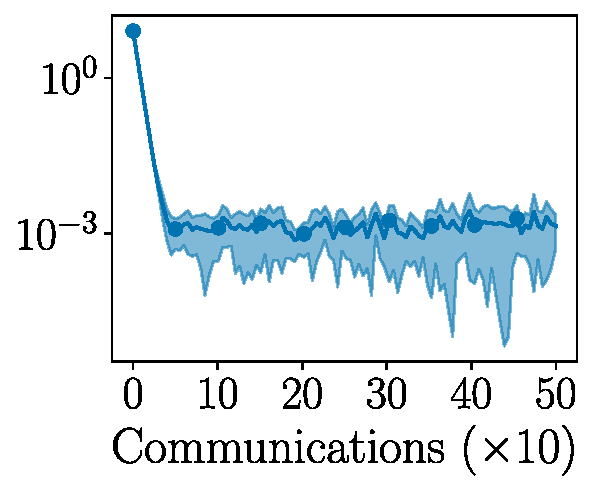
\includegraphics[width=0.4\linewidth]{plots/plot_hm_fedlsa.pdf}
  \end{center}

\end{frame}

\begin{frame}[t]
  \vspace{1em}

  Biased if agents are heterogeneous ($H=1000$)

  \begin{center}
    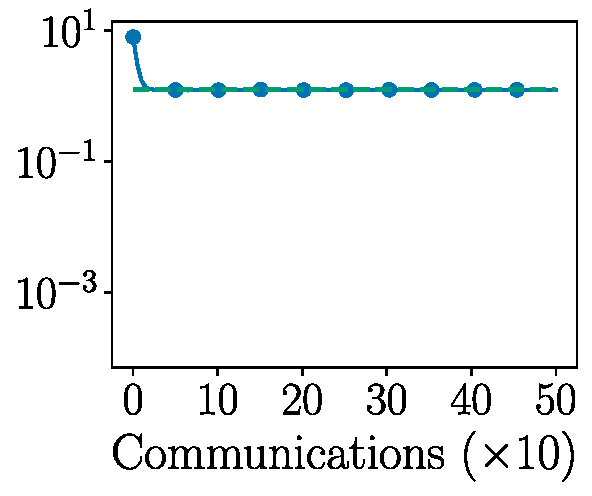
\includegraphics[width=0.4\linewidth]{plots/plot_hg_fedlsa.pdf}
  \end{center}

  $\rightarrow$ and we can give a formal expression of this bias

  $\rightarrow$ if $\eta$ and $H$ are small, then bias is also small!
\end{frame}

\begin{frame}
  { \Large SCAFFLSA: Use Control Variates! }
  \begin{itemize}
  \item Initialize $\theta_0$, $\xi_0^1$, $\dots$, $\xi_0^N$
  \item For $t = 0$ to $T-1$:
    \begin{itemize}
    \item Set $\theta_{t,0}^c = \theta_{t}$
    \item For each agent $c$, for $h=0$ to $H-1$:

      \vspace{-1em}
      
      
      \begin{align*}
        \theta_{t,h}^c - \eta ( A^c(Z_{t,h+1}^c) \theta_{t,h}^c - b^c(Z_{t,h+1}^c) - \xi_t^c)
      \end{align*}

      \vspace{0.5em}

    \end{itemize}
    \item Aggregate $\theta_{t+1} = \frac{1}{N} \sum_{c=1}^N \theta_{t,H}^c$
    \item Update $\xi^c_{t+1} = \xi_t^c + \frac{1}{\eta H} ( \theta_{t+1} - \theta_{t,H}^c )$
  \end{itemize}  
\end{frame}

\begin{frame}
  Works even if agents are heterogeneous ($H=1000$)

  \begin{center}
    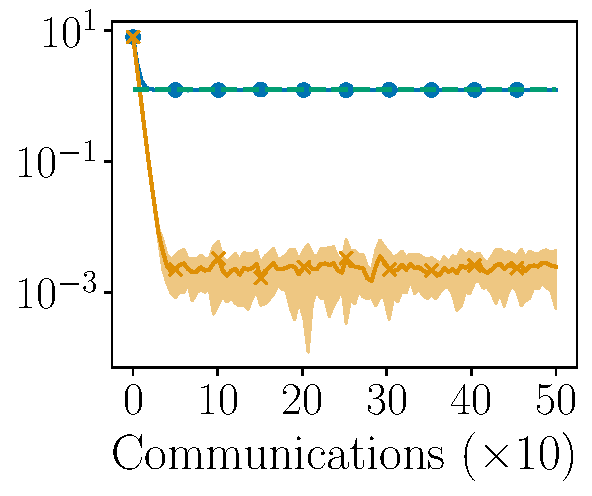
\includegraphics[width=0.4\linewidth]{plots/plot_hg_scafflsa.pdf}
  \end{center}

\end{frame}

\begin{frame}
  \begin{table}
        \renewcommand{\arraystretch}{1.5}
        \small
    \centering 
    \begin{tabular*}{1\textwidth}{@{\extracolsep{\fill}} ccccc }
      %\begin{tabular}{ccccc}
    \toprule
        Algorithm & 
        Communication $T$ &
        Local updates $H$ &
        Total samples 
    \\
    \midrule
         FedLSA
         &
          $\displaystyle\mathcal{O} \left({\tfrac{1}{ a^2 \epsilon}} \log{\tfrac{1}{\epsilon}} \right)$
         &
         $\displaystyle\mathcal{O} \bigl( \tfrac{1}{N \epsilon}\bigr)$
         &
         $\displaystyle\mathcal{O}\bigl(\tfrac{1}{ N a^2 \epsilon^2} \log{\tfrac{1}{\epsilon}}\bigr)$
    \\
        Scafflsa &
        $\displaystyle\mathcal{O}\left( \tfrac{1}{a^2} \log \tfrac{1}{\epsilon}\right)$
        & 
        $\displaystyle\mathcal{O}\bigl(\tfrac{1}{N \epsilon^2} \bigr)$
        &
        $\displaystyle\mathcal{O}\bigl(\tfrac{1}{ N a^2 \epsilon^2} \log{\tfrac{1}{\epsilon}}\bigr)$
    \\
    \bottomrule
    \end{tabular*}
%    \vspace{-2em}
  \end{table}

  Important new results:
  \begin{itemize}
  \item linear speed-up with control variates
  \item acceleration in the setting where noise dominates
  \end{itemize}
\end{frame}

\begin{frame}
  \begin{center}
    
    \large
    Thank you, see you in Vancouver! :)

    \vspace{2em}

    \large
    Poster session:
    
    \textcolor{purple}{\textbf{Fri 13 Dec 4:30 p.m. — 7:30 p.m. PST}}
  \end{center}
\end{frame}

\end{document}

%%% Local Variables:
%%% mode: latex
%%% TeX-master: t
%%% End:
